\section{Introduction}

All Lorentz transformations have two inherent null directions, except the singular Lorentz transformations \cite[p. 85]{Relativity_Synge}. The Lorentz Transform is defined by $(x,y,z,t) \rightarrow (x',y',z',t')$ such that

\begin{equation*}
{x'}^2 + {y'}^2 + {z'}^2 - {t'}^2 = x^2 + y^2 + z^2 - t^2.
\end{equation*}

\noindent If the transformation preserves the orientation of the spatial axes then is it called a \textit{proper} Lorentz transformation, this is equivalent to taking the subgroup of the Lorentz group of transformations with determinant $1$. This is also understood as the preservation of the handedness of the axes. If determinant $-1$ was chosen a reflection in some spacial axis, $x^j = -{x'}^j$ would also give a proper Lorentz transformation. If $t \geq 0$ implies that time is always positive then it is called an \textit{orthochronous} Lorentz transformation, which ensures that the time direction is preserved. In this project the ``Lorentz transformation'' will refer to the proper, orthochronous Lorentz transformation.

\begin{figure}[h!]
\begin{center}
\caption{\textit{Space-Time Diagram for a photon moving at the speed of light, $c=1$ and starting from $x = 0$. Two null directions can be seen.}}
\label{figure_Photon_Space_Time}
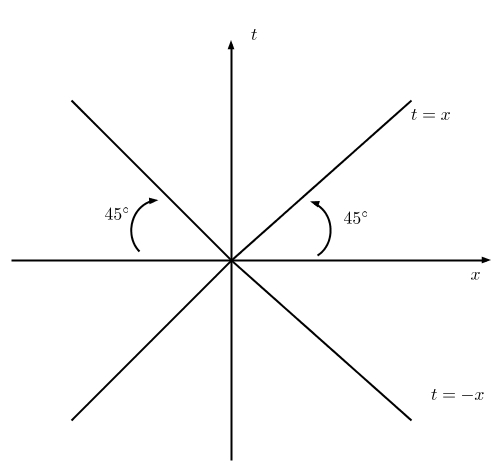
\includegraphics[scale=0.8]{figs/1_1.jpg}
\end{center}
\end{figure}

Consider a photon moving in the $x$ direction at the speed of light, $c = 1$, and starting at $x = 0$. The space-time for such a photon can be illustrated as in Fig.(\ref{figure_Photon_Space_Time}). It is clear that there are two null directions in this space-time, $x = \pm t$. To see this use the standard Lorentz transformation

\begin{align*}
x'  = \gamma (x - vt),  \\
t'  = \gamma (t - vx),
\end{align*}

\noindent where $\gamma = {(1 - v^2)}^{-1/2}$. Rearrange to obtain

\begin{eqnarray*}
x' - t' = \gamma (1 + v) (x - t), \\
x' + t' = \gamma (1 - v) (x + t).
\end{eqnarray*}

\noindent It is clear that $x = \pm t$ implies $x' = \pm t'$. Thus there are two null directions in this space-time at $x = \pm t$, as null directions are by definition invariant under a Lorentz transformation. It can be shown that all Lorentz transformations have two invariant null directions except the singular Lorentz transformation which has only one fixed null direction.  
